%introduction
\section{Introduction}
\justify
In this laboratory assignment we will be working with heat diffusion algorithms, specially with Jacobi and Gauss-Seidel approaches.

\justify
What these algorithm does is given a number of heat focus in a 2D coordinate space, it simulates it's diffusion, getting the following results.

\begin{figure}[h!]
    \centering
    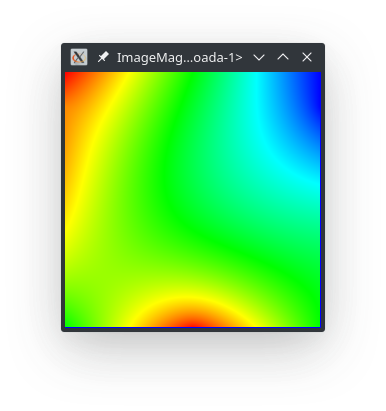
\includegraphics[width=0.55\textwidth]{heat.png}
    \caption{Heat diffusion results}
    \label{fig:heat1}
\end{figure}

\justify
First of all we will be working with Jacobi algorithm because it's parallelization it's a bit simple and we will get better in touch with heat diffusion algorithms as it's approach has differences but is similar. Later on we will introduce Gauss-Seidel approach which has a different approach.

